% Chapter 11

\chapter{Comparación Modelo de la ANN} % Write in your own chapter title
\label{Chapter12}
\lhead{Capítulo 12. \emph{Comparación ANN}} % Write in your own chapter

En este capítulo se analizará comparativamente los niveles de detección entre un modelo de Red Neuronal Artificial usando las herramientas de Matlab (nntool) y el modelo en hardware propuesto en este documento en el Capítulo \ref{Chapter6}, figura \ref{fig:MLP}. El objetivo es demostrar que el modelo propuesto es válido y puede ser implementado a nivel de hardware directamente, para esto se eligió mostrar la detección del modelo de la red en punto fijo usando el entrenamiento de Matlab con especificaciones iguales a las del modelo Hardware propuesto, también se usó el entrenamiento directamente sobre el modelo hardware usando C/C++ y finalmente se eligó usar los pesos encontrados usando el entrenamiento de Matlab sobre los pesos del modelo Hardware.

\begin{figure}[H]
	\centering
		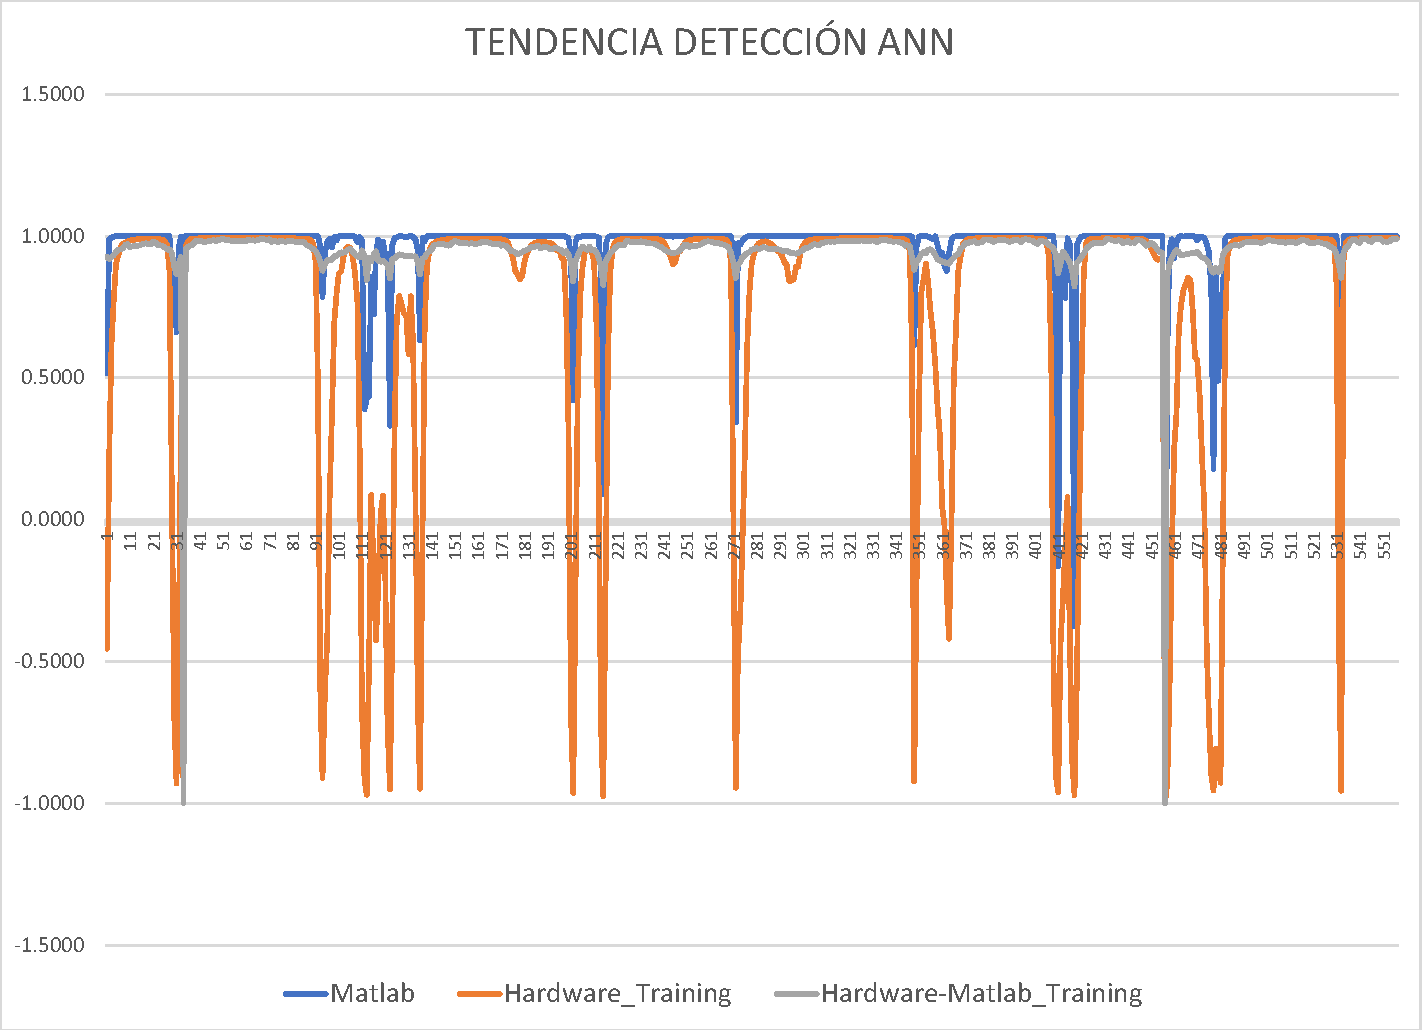
\includegraphics[scale=0.6]{./Figures/TendenciaANN1}
	\caption{Detección de la ANN Positivo}
	\label{fig:TendP}
\end{figure}

 Las figuras \ref{fig:TendP} y \ref{fig:TendN}, muestran el rendimiento de la red neuronal al detectar o no una posible inundación basado en el entrenamiento y el set de datos elegido. Se observa que el modelo entrenado directamente usando el Hardware (color naranja) presenta más falsos Negativos que el modelo implementado usando Matlab (color azul), también se observa que al usar los pesos sinápticos encontrados con el entrenamiento usando Matlab sobre el modelo Hardare (color gris) presenta un rendimiento similar al modelo de Matlab. Tambien se observa que el modelo Matlab presenta varios falsos Positivos al igual que el modelo Hardware con los pesos encontrados usando Matlab.
 


\begin{figure}[H]
	\centering
		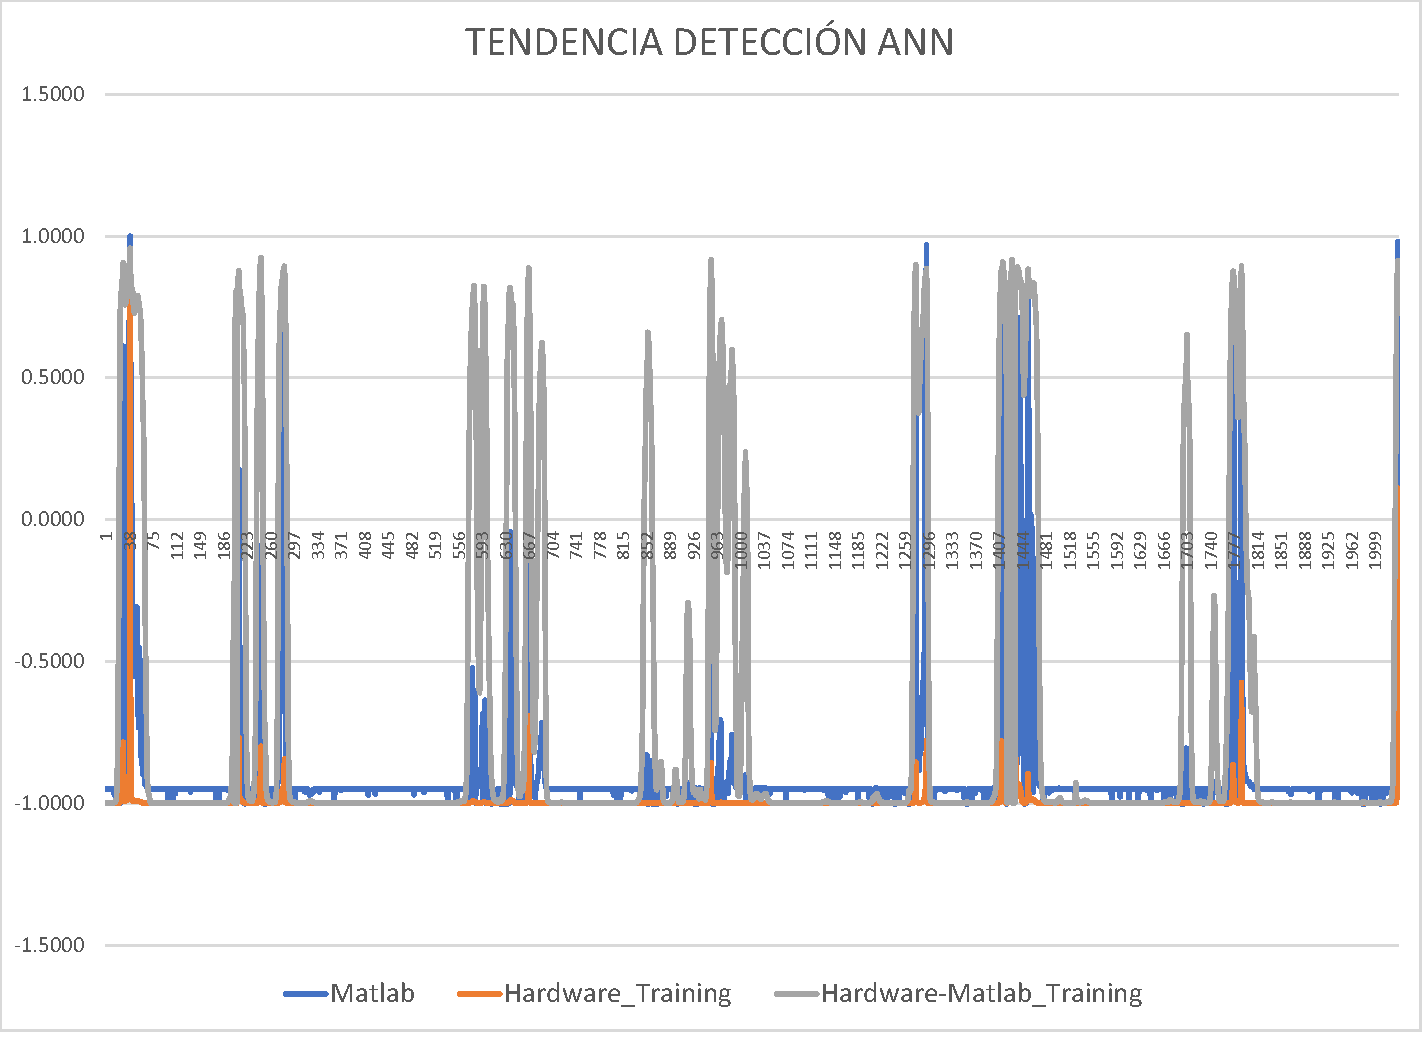
\includegraphics[scale=0.6]{./Figures/TendenciaANN2}
	\caption{Detección de la ANN Negativo}
	\label{fig:TendN}
\end{figure}

 La figura \ref{fig:DistP} muestra como se encuentran distribuidos los valores de detección Positiva de los modelos, en este caso observamos que el modelo Matlab presenta una distribución muy compacta de los datos con algunos valores atípicos. El modelo Hardware usando los pesos encontrados usando Matlab presenta una distribución de los datos poco menos compacta que el modelo de Matlab pero con datos atípicos más cercanos al valor del detección establecido en el entrenamiento.

\begin{figure}[H]
	\centering
		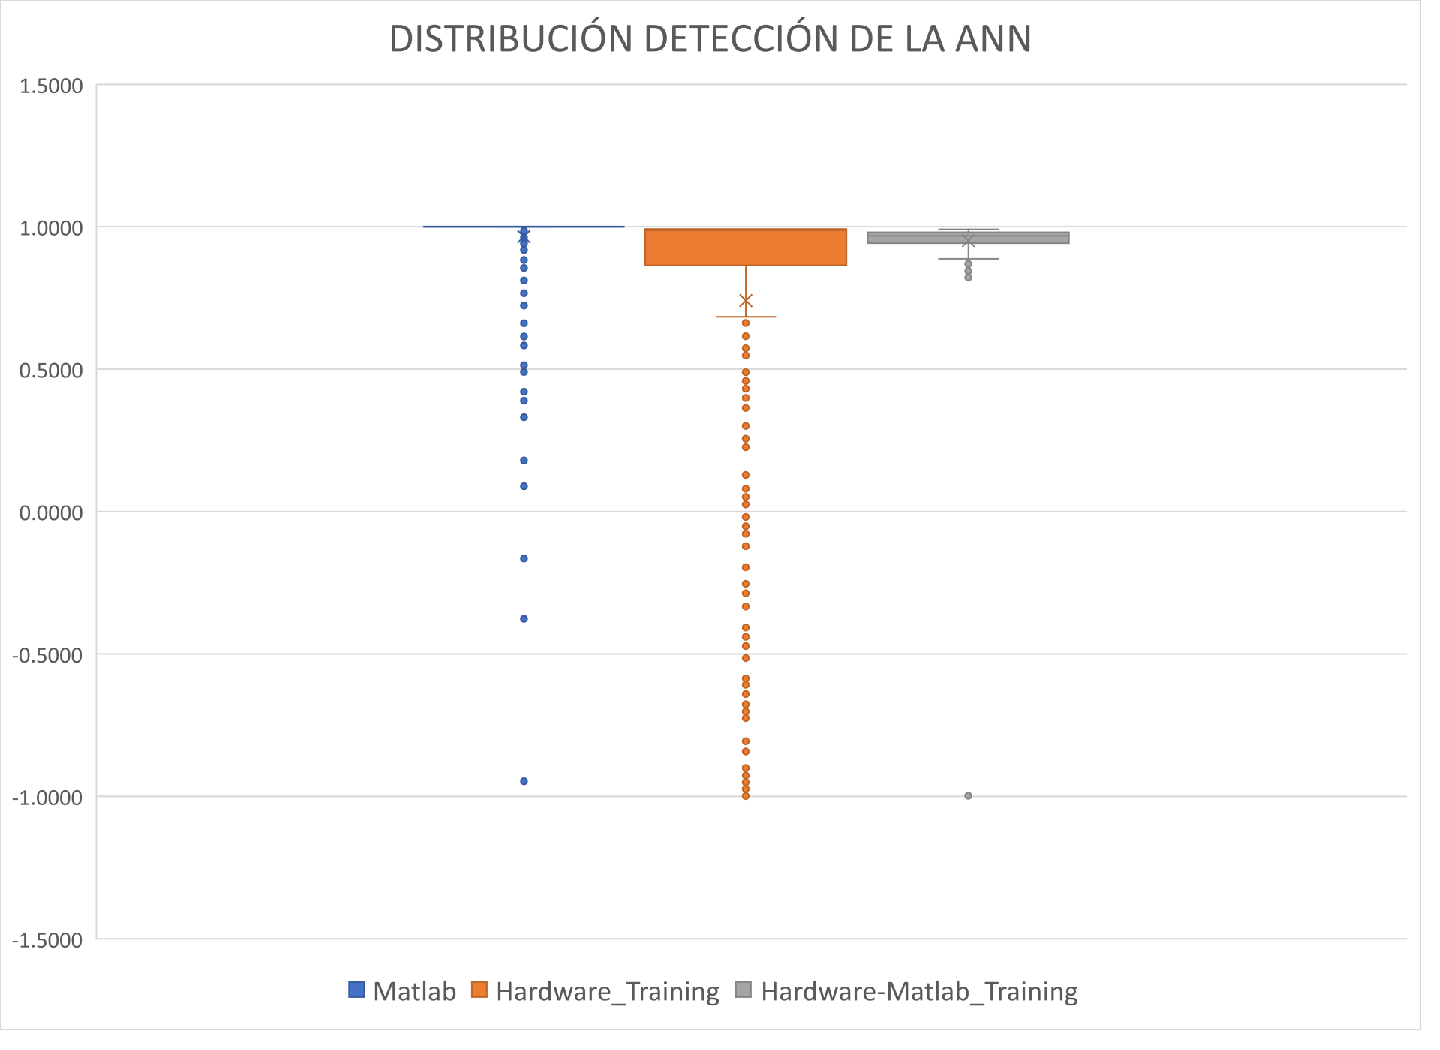
\includegraphics[scale=0.6]{./Figures/Distribucion1}
	\caption{Distribución de la detección Positivo}
	\label{fig:DistP}
\end{figure}

Finalmente la figura \ref{fig:DistN} muestra la distribución de detección negativa del set de datos, aqui se observa que el entrenamiento de la red directamente sobre el Hardare presenta un mejor rendimiento al observar que los datos se encuentran más compactos sobre el nivel negativo de detección $-1$ con la media directamente sobre este nivel.

\begin{figure}[H]
	\centering
		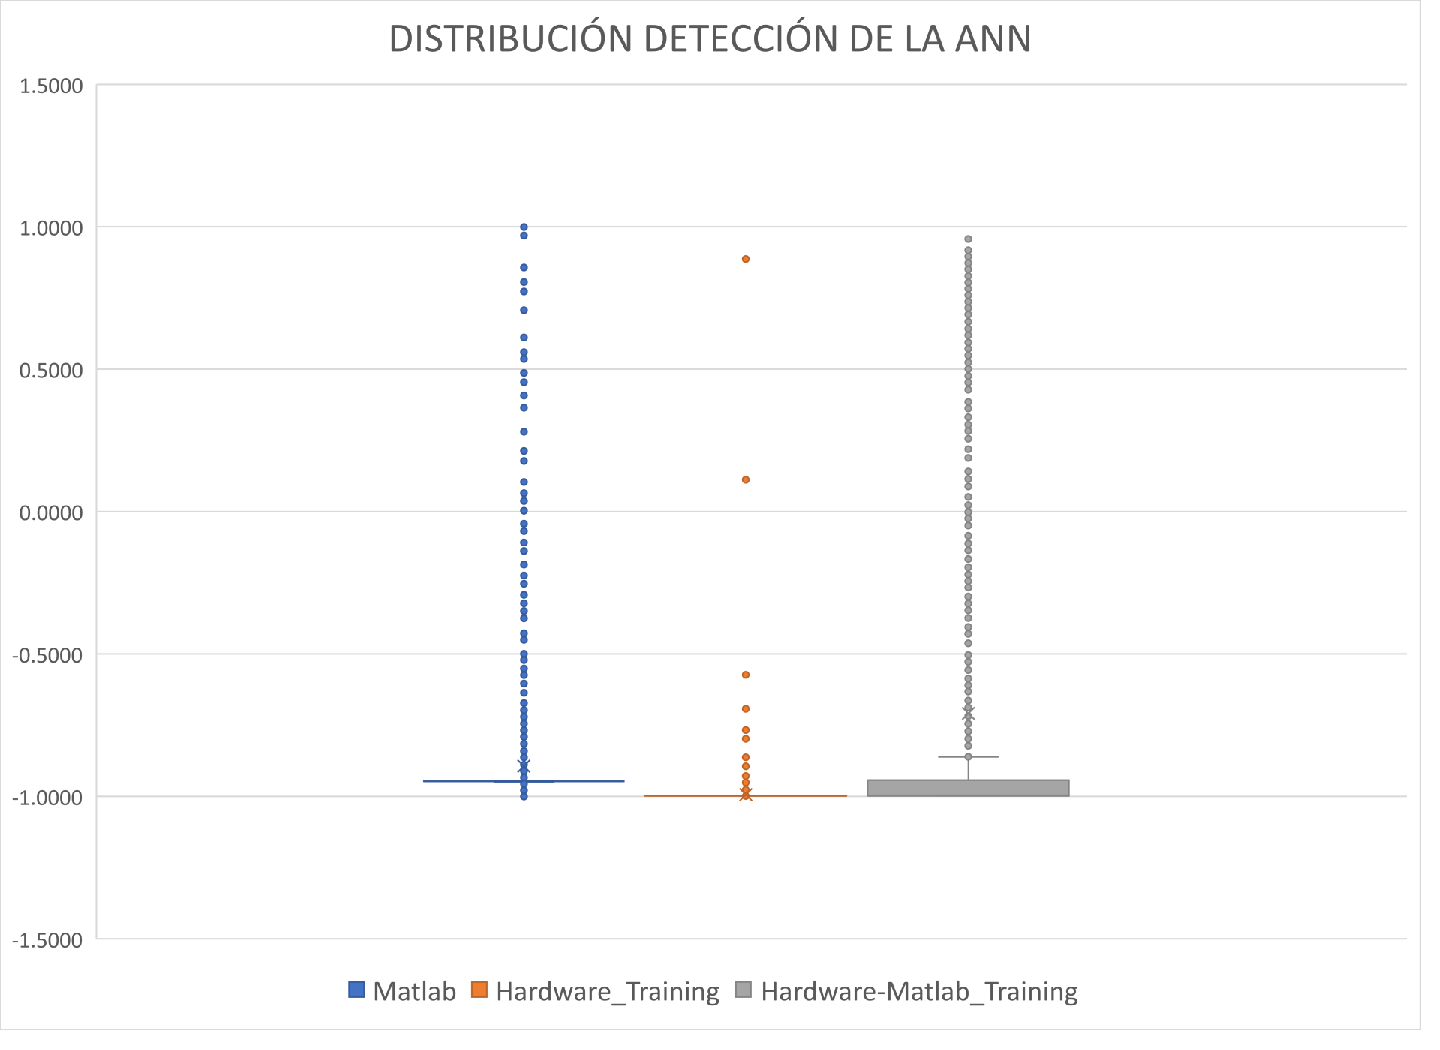
\includegraphics[scale=0.6]{./Figures/Distribucion2}
	\caption{Distribución de la detección Negativo}
	\label{fig:DistN}
\end{figure}

Con estos datos es posible determinar que la implementación en Hardware es correcta y que funcionalmente se encuentra en capacidad de detectar eficazmente la probabilidad de inundación en comparación con un modelo netamente Software como el propuesto usando las herramientas de Matlab.

Es importante mencionar que el rendimiento de ambas redes tanto la propuesta usando Matlab como la desarrollada en Hardware dependende directamente de la calidad del entrenamiento y el set de datos elegido, es de notar que ambos casos presentan falsos positivos y negativos, pero esto se debe en gran parte a los valores que se encuentran en las transiciones de un valor normal para el río a una posible inundación.

Los resultados de detección para la red neuronal aquí expuestos implican que es posible usar configuraciones de redes neuronales mucho más complejas que en Matlab son muy simples de configurar y que los resultados del entrenamiento puedan ser llevados a la implementación Hardware sin dudas que la variación en la detección cambie drásticamente sin necesidad de implementar complejos algoritmos de entrenamiento usando C/C++ directamente sobre el hardware como aquí se propuso.